\documentclass[conference]{IEEEtran}
\usepackage[T1]{fontenc}
\usepackage{booktabs}
\usepackage{graphicx}
\usepackage{amsmath,amssymb}
\usepackage{array}
\usepackage{url}
\usepackage{hyperref}
\usepackage{enumitem}
\usepackage{microtype}
\usepackage{balance}
\setlist[itemize]{leftmargin=*,nosep}
\begin{document}
\pagestyle{empty}

\title{Predicting, Quantifying, and Explaining Sprint Outcomes from Reconstructed Jira Histories}

\author{\IEEEauthorblockN{Hani AbuSharkh}
\IEEEauthorblockA{Higher Colleges of Technology\\United Arab Emirates\\habusharkh@hct.ac.ae}
\and
\IEEEauthorblockN{Maryam Hanif}
\IEEEauthorblockA{United Arab Emirates University\\United Arab Emirates\\700052696@uaeu.ac.ae}
\and
\IEEEauthorblockN{Rafat Damseh}
\IEEEauthorblockA{United Arab Emirates University\\United Arab Emirates\\rdamseh@uaeu.ac.ae}}
\maketitle
\thispagestyle{empty}

\begin{abstract}
Repository data are useful at Sprint Planning only if the features reflect what the team knew at that time.
We reconstruct sprint-start state from Jira change histories in eight open-source TAWOS projects (2,602 modeled sprints, 1,691 with committed scope) and study five prediction tasks: two binary---late sprint closure and unfinished committed scope (spillover)---and three numeric---issues completed, share of scope carried over, and days closed late.
We compare baselines, logistic regression, random forest, and gradient boosting under per-project chronological splits and leave-one-project-out (LOPO) cross-validation, with project-cluster bootstrap intervals (2,000 resamples).

Two findings anchor the analysis.
First, the two binary outcomes respond to different signals: spillover is dominated by initial scope (a scope-only logistic model reaches ROC-AUC 0.885, outperforming richer models), while late closure depends on project identity and team history (gradient boosting with strict history features reaches 0.751).
Second, history features that account for parallel-sprint timing---ensuring that only sprints whose outcomes were already known contribute to the feature vector---improve late-closure AUC by 0.025 to 0.087 depending on model and protocol, while leaving spillover rankings essentially unchanged.

Exact Shapley values per feature group confirm these patterns quantitatively: past lateness (38\%) and project (22\%) explain late closure, while scope alone accounts for 71\% of the issues-completed prediction.
A sprint advisor built on the fitted models produces 80\% prediction intervals for issues completed that cover 84--85\% of outcomes and are a third narrower than the scope-times-rate baseline, and 90th-percentile late-days forecasts that are exceeded about 10\% of the time.
However, observational what-if tables show no significant causal effect of reducing scope on either carryover share or late-closure probability across the eight projects.
The analysis supports retrospective understanding, not deployment-ready advice.
\end{abstract}

\begin{IEEEkeywords}
Scrum, sprint analytics, Jira, machine learning, explainability, data leakage
\end{IEEEkeywords}

%% ================================================================
\section{Introduction}
Sprint Planning is one of the few points in Scrum where the team can still reshape the work before execution begins.
By the time a burndown stalls or unfinished items accumulate in the Daily Scrum, options have narrowed.
This makes the sprint-start moment a natural cutoff for any prediction system that aims to inform planning rather than merely describe outcomes after the fact.

Existing sprint-level prediction studies vary in how strictly they enforce this cutoff.
Some use burndown data collected during the sprint~\cite{perezcastillo2024};
others report features that should in principle be available at planning time but do not reconstruct the historical state of fields that change after the sprint starts~\cite{obike2025}.
Neither approach guarantees that a model trained on ``planning-time'' features could have been applied at the actual planning meeting.
Projects also frequently run sprints in parallel: on average 1.9 other sprints are already in progress when a sprint starts in our data, and in 71\% of cases a sprint begins before the previous one is supposed to end.
History features that summarize the ``prior sprint'' can therefore leak information from sprints whose outcome was not yet known.

We address five research questions on the TAWOS dataset~\cite{tawosi2022}, using Sprint, Issue, and Change\_Log tables from eight open-source Jira projects:

\begin{enumerate}[leftmargin=*,nosep,label=\textbf{RQ\arabic*.}]
\item How much ranking signal do reconstructed sprint-start features carry for late closure and spillover?
\item Does a simple scope-only model perform comparably to richer models?
\item Do strict history features that respect parallel-sprint timing improve predictions over legacy features that ignore it?
\item What drives each outcome? Which feature groups explain the model's behavior?
\item Can these models produce useful numeric forecasts---predicted issues completed, carryover share, days late---with calibrated uncertainty?
\end{enumerate}

Our contributions are:
(a) a reconstruction pipeline that rebuilds Sprint membership and Story Points from timestamped change records, with documented static fallback and provenance reporting;
(b) strict history features that only draw on sprints whose outcome was known at the current sprint's start, plus parallel-sprint count, team capacity, and past lateness;
(c) numeric outcome models alongside the binary classifiers, evaluated under the same time split and LOPO protocols;
(d) exact Shapley values decomposing each model's output into feature-group contributions;
(e) a sprint advisor that translates the fitted models into prediction intervals and what-if tables, with explicit tests of whether those tables describe a causal relationship;
and (f) controlled leakage demonstrations and provenance-sensitivity analyses that show how evaluation choices and data quality interact with the headline numbers.

%% ================================================================
\section{Related Work}

Machine learning in Agile software analytics has been applied to effort estimation, sprint monitoring, and project-risk support.
Choetkiertikul et al.~\cite{choetkiertikul2019} estimated story points from Jira text using a deep learning architecture.
Tawosi et al.~\cite{tawosi2023} replicated and extended that work on the TAWOS dataset, finding that simpler models often match deep learning when the feature set is held constant, a finding consistent with our observation that scope-only logistic regression rivals more complex classifiers for spillover.
Shankar et al.~\cite{shankar2026} compared several predictive models for Agile effort data and found gradient-boosted methods competitive.

On sprint-level outcomes, P\'{e}rez Castillo et al.~\cite{perezcastillo2024} classified sprint performance using burndown information observed during the sprint.
Obike et al.~\cite{obike2025} predicted sprint deliverability with an ensemble method, though the features were described as planning-time without reconstruction from change history.
Almalki~\cite{almalki2025} examined interpretable AI for Agile project-risk support using historical project data.

The explainability side of our work draws on Lundberg and Lee's~\cite{lundberg2017} unified framework for Shapley-based feature attribution.
Rather than using the SHAP library's kernel or tree approximations, we compute exact Shapley values over seven feature groups (at most $2^7 = 128$ coalitions), which is tractable for our feature-group structure and avoids approximation error.
Molnar~\cite{molnar2022} provides a comprehensive treatment of interpretable machine-learning methods, including the distinction between feature importance (a global summary) and Shapley values (instance-level, additive attribution).

The key gap our work addresses is the combination of sprint-start reconstruction, cross-project evaluation, and quantitative explanation.
Table~\ref{tab:related} compares the studies above on what is predicted, when the inputs are captured, and whether evaluation holds out whole projects.

\begin{table}[!htb]
\centering\scriptsize
\caption{Selected related work and the evaluation gap}
\label{tab:related}
\setlength{\tabcolsep}{1.8pt}
\begin{tabular}{@{}p{1.3cm}p{1.4cm}p{1.1cm}p{0.9cm}p{1.0cm}@{}}
\toprule
Study & Main task & Sprint-start features & Project holdout & Explanations\\
\midrule
Choetkiertikul et al. & Story-point estimation & Yes & No & No\\
Tawosi et al. (2023) & Effort replication & Yes & Partial & No\\
Shankar et al. & Effort/time & Yes & No & No\\
P\'{e}rez Castillo et al. & Sprint perf. & No; burndown & No & No\\
Obike et al. & Deliverability & Intended & No & No\\
Almalki & Risk support & Historical & No & Partial\\
\textbf{This work} & \textbf{Closure / scope / numeric} & \textbf{Reconstructed} & \textbf{Yes (LOPO)} & \textbf{Shapley}\\
\bottomrule
\end{tabular}
\end{table}

%% ================================================================
\section{Data and Reconstruction}

We use eight open-source projects from TAWOS~\cite{tawosi2022}, each with at least 30 sprint records.
The selected projects give us 2,657 sprint rows and 145,309 issues.
Table~\ref{tab:flow} shows how the rows are filtered before modeling.
FUTURE and ACTIVE rows are removed because their closure outcome is not observed.
Three CLOSED rows with impossible timestamps (close time before start) are also removed.
Historical features require a predecessor, so the first eligible sprint in each project is the only cold start excluded.
After these exclusions, 2,602 sprints remain for modeling; 1,691 of those have at least one committed issue and constitute the nonempty population used for spillover and numeric-outcome analyses.

\begin{table}[!htb]
\centering\scriptsize
\caption{Sprint flow by project}
\label{tab:flow}
\setlength{\tabcolsep}{2.1pt}
\begin{tabular}{@{}p{2.0cm}rrrrr@{}}
\toprule
Project & Raw & Nonclosed & Invalid & Modeled & Nonempty\\
\midrule
Apache Mesos & 227 & 2 & 0 & 224 & 133\\
Appcelerator Studio & 163 & 0 & 0 & 162 & 129\\
Confluence Cloud & 477 & 10 & 2 & 464 & 197\\
Confluence Server & 565 & 7 & 0 & 557 & 289\\
Lsstcorp Data & 396 & 8 & 0 & 387 & 309\\
Mule & 311 & 13 & 0 & 297 & 228\\
Titanium SDK & 301 & 1 & 0 & 299 & 241\\
Titanium Mobile & 217 & 3 & 1 & 212 & 165\\
\bottomrule
\end{tabular}
\end{table}

TAWOS uses two different sprint identifiers: the database ID and the Jira sprint ID.
We build project-level maps for both before tracing issue history.
Starting from the latest recorded state, the code walks each issue's changes backward to the sprint-start time.
An issue is included in the committed set only if it already existed, belonged to that sprint at that time, and was not resolved before the start.
Story Points are reconstructed in the same way.
This produces 20,603 issue-sprint commitments across the eligible sprints.

Not every issue has a recorded Sprint or Story Points change.
When a change is missing, we fall back to the static value and treat it as unchanged---an assumption the data cannot confirm.
Since coverage differs across projects (Table~\ref{tab:provproj}), we report the provenance of the commitments and rerun the analysis on subsets with observed history (Section~\ref{sec:provenance}).

\begin{table}[!htb]
\centering\scriptsize
\caption{Commitment provenance by project}
\label{tab:provproj}
\setlength{\tabcolsep}{2.2pt}
\begin{tabular}{@{}p{2.0cm}rrr@{}}
\toprule
Project & Sprint hist. & Sprint fallback & SP hist.\\
\midrule
Apache Mesos & 96.4\% & 3.6\% & 56.8\%\\
Appcelerator & 95.8\% & 4.2\% & 87.2\%\\
Confluence Cloud & 54.1\% & 45.9\% & 11.2\%\\
Confluence Server & 99.1\% & 0.9\% & 54.4\%\\
Lsstcorp Data & 92.4\% & 7.6\% & 41.8\%\\
Mule & 92.3\% & 7.7\% & 77.0\%\\
Titanium SDK & 97.1\% & 2.9\% & 68.3\%\\
Titanium Mobile & 93.6\% & 6.4\% & 54.0\%\\
\bottomrule
\end{tabular}
\end{table}

\subsection{Parallel sprints and the history-timing problem}

Projects in our data frequently run multiple sprints concurrently.
On average, 1.9 other sprints are already in progress when a sprint starts, with a maximum of 11 concurrent sprints.
In 71\% of cases, a sprint begins before the previous sprint's planned end date.
This means that a feature labeled ``prior sprint completion ratio'' may reference a sprint whose outcome was not yet known at planning time, introducing a subtle form of temporal leakage.

We define two feature sets.
The \emph{legacy} set mirrors the original Phase~1 features: it summarizes the immediately preceding sprint regardless of whether that sprint had finished.
The \emph{strict} set restricts historical summaries to sprints whose completion date falls before the current sprint's start, and adds three new feature groups: the number of sprints running in parallel, the team's recent capacity (issues completed per sprint among recently finished sprints), and past lateness (the fraction of recently completed sprints that closed late).
Both sets share the same current-sprint predictors (committed issues, committed story points, and sprint length) and project identity.

\begin{figure}[t]
\centering
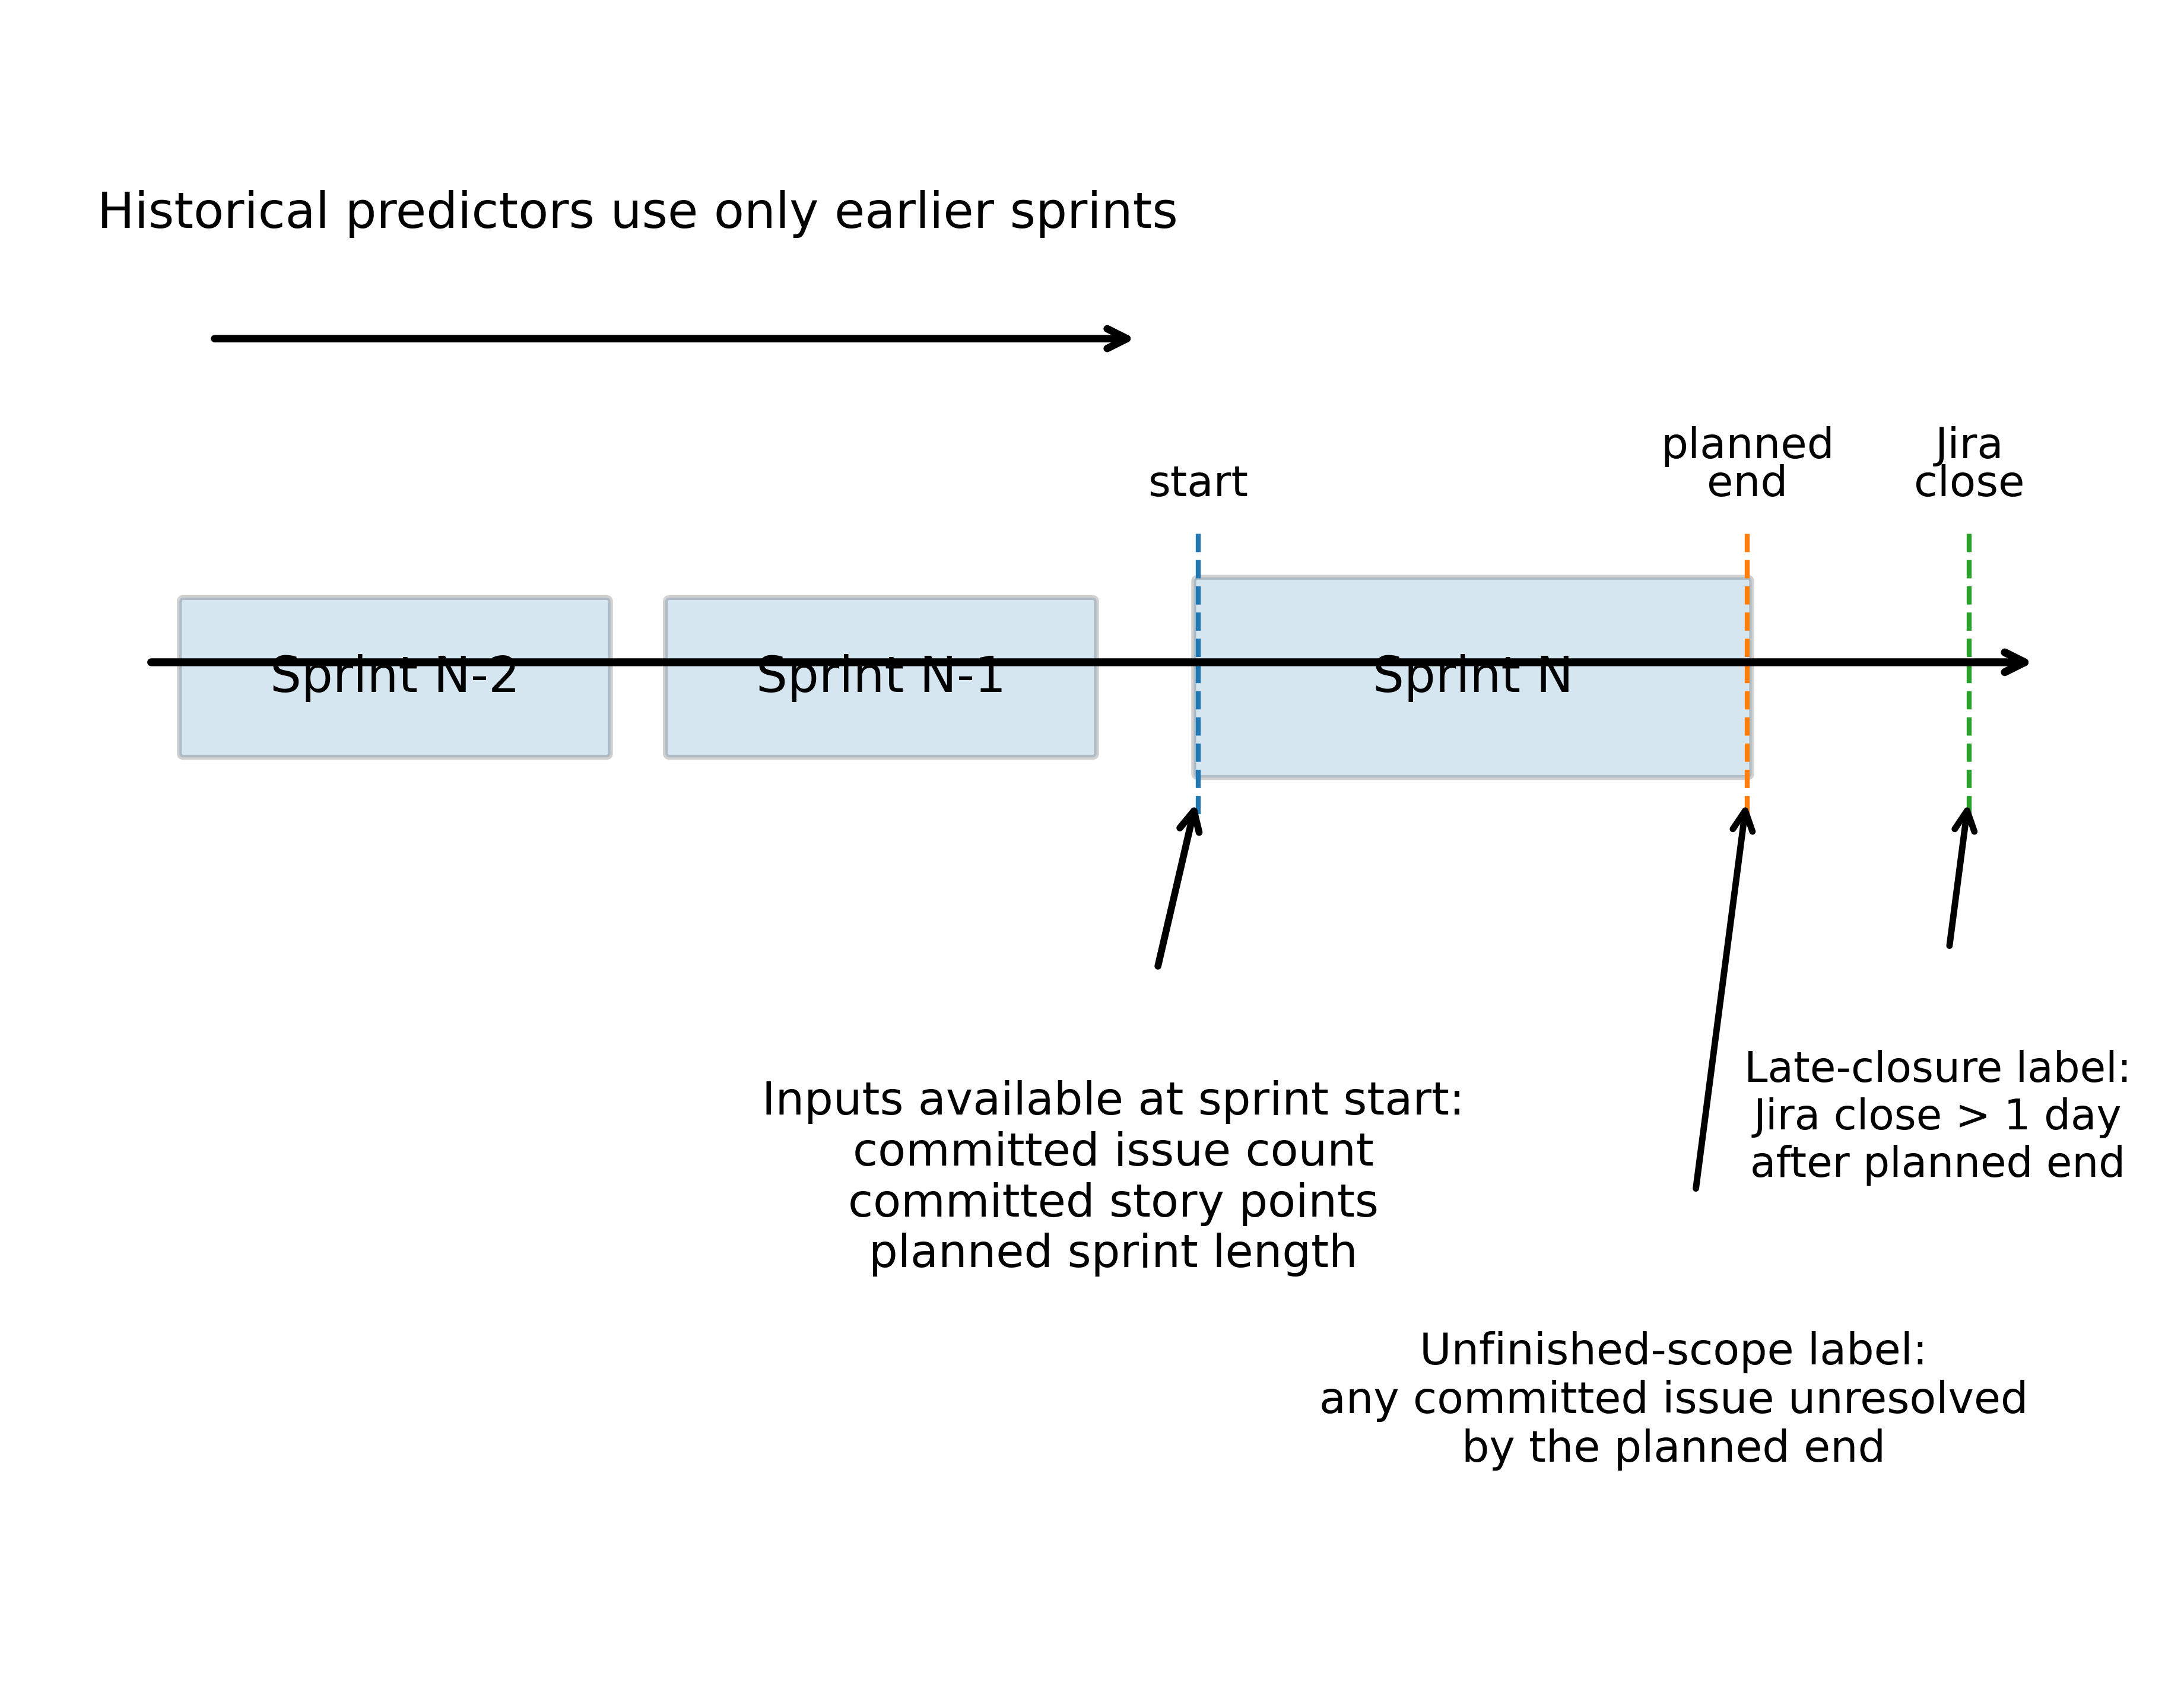
\includegraphics[width=0.93\columnwidth]{dataflow_timing_clean.png}
\caption{Data timing and reconstruction used before model fitting.}
\label{fig:dataflow}
\end{figure}

%% ================================================================
\section{Methods}

\subsection{Outcomes}
We study five prediction tasks on two populations.

\emph{Binary outcomes.}
Late closure is $y^{late}_s = \mathbb{1}[c_s - e_s > 1\text{ day}]$,
where $c_s$ is Jira's completion timestamp and $e_s$ is the planned end.
Spillover is $y^{spill}_s = \mathbb{1}[u_s > 0]$,
where $u_s$ is the count of sprint-start committed issues unresolved at the planned end.
Late closure uses all 2,602 modeled sprints; spillover uses the 1,691 nonempty sprints.

\emph{Numeric outcomes.}
Issues completed ($\hat{d}_s$): how many committed issues are resolved by the planned end.
Carry share ($\hat{r}_s$): the fraction of committed issues not completed, $u_s / n_s$.
Days late ($\hat{\ell}_s$): $\max(0, c_s - e_s)$ in days, capped at 30.
All three use the nonempty population except days late, which uses the full cohort.

\subsection{Features}
\begin{table}[!htb]
\centering\scriptsize
\caption{Feature groups used in the analysis}
\label{tab:features}
\setlength{\tabcolsep}{2.0pt}
\begin{tabular}{@{}p{1.6cm}p{4.0cm}p{0.7cm}@{}}
\toprule
Group & Variables & Sets\\
\midrule
Scope & committed issue count; committed story points & Both\\
Sprint length & planned duration in days & Both\\
Recent history & mean delivered points, mean completion ratio, prior carryover, prior completion ratio (over recently finished sprints) & Both\textsuperscript{$\dagger$}\\
Parallel sprints & count of other in-progress sprints at start & Strict\\
Capacity & team's mean issues completed per recent sprint & Strict\\
Past lateness & fraction of recent sprints that closed late & Strict\\
Project & one-hot project identity & Both\\
\bottomrule
\multicolumn{3}{@{}l@{}}{\textsuperscript{$\dagger$}\scriptsize Legacy: ``recent'' = immediately prior sprint (may be unfinished).}\\
\multicolumn{3}{@{}l@{}}{\scriptsize Strict: only sprints completed before current start.}
\end{tabular}
\end{table}

\subsection{Models and baselines}
For binary outcomes, we compare: always-positive and project-base-rate baselines; scope-only logistic regression (committed issues, committed story points, sprint length); logistic regression with all features; random forest (300 trees, max depth~5, min leaf~3, balanced weights); and gradient boosting (300 trees, max depth~4, learning rate~0.05).
Precision, recall, and F1 use a fixed 0.5 threshold.
ROC-AUC is the primary ranking metric.

For numeric outcomes, we compare: train-mean and train-median baselines; a scope-times-rate baseline (committed issues $\times$ historical completion rate, for issues completed); a prior-history baseline (most recent sprint's value); ridge regression; random forest; gradient boosting; and a gradient booster trained on median (quantile) loss.
Mean absolute error (MAE) is the primary metric; $R^2$ and Spearman correlation are secondary.

\begin{table}[!htb]
\centering\scriptsize
\caption{Model settings held fixed across the reported runs}
\label{tab:settings}
\setlength{\tabcolsep}{2.4pt}
\begin{tabular}{@{}p{1.65cm}p{5.1cm}@{}}
\toprule
Model & Main settings\\
\midrule
Logistic regression & standardized numeric features; balanced class weights\\
Ridge regression & standardized numeric features; default regularization\\
Random forest & 300 trees; max depth 5; min leaf 3; balanced weights\\
Gradient boosting & 300 trees; max depth 4; LR .05; log-loss (classif.)\ or squared-error (regress.)\ objective\\
GB median & same as above but quantile loss ($\alpha = 0.5$)\\
\bottomrule
\end{tabular}
\end{table}

\subsection{Validation}
For the main test, we order each project's sprints chronologically and train on the earlier 70\%, testing on the later 30\%.
In leave-one-project-out (LOPO) testing, we hold out one entire project and train on the other seven.
Historical features for the held-out project are still computed from its own earlier sprints, so LOPO measures how well the learned rule transfers, not a complete cold start.
For uncertainty, we resample projects as whole units (2,000 bootstrap replicates) rather than individual sprints.

\subsection{Shapley explanations}
We compute exact Shapley values at the feature-group level.
With seven groups, the power set has $2^7 = 128$ coalitions, each trained and evaluated as a separate model---tractable, and free of approximation error.
For each coalition, we retrain the model using only the features in that group subset, evaluate on the test set, and compute the marginal contribution of each group across all coalitions in which it appears.
The resulting attributions are additive: they sum to the difference between the full model's metric and the empty model's.
We report the mean absolute Shapley attribution as each group's importance share.

\subsection{Sprint advisor}
The advisor wraps the fitted models into a planning-time tool.
For a given committed scope, it reports: expected issues completed with an 80\% prediction interval (from the quantile-loss model's 10th and 90th percentile forecasts); expected carryover share; the probability of any spillover (from the classification model's predicted probability); the probability of late closure; and the median and 90th-percentile forecast of days late.
A what-if table varies the committed scope and reports how each forecast changes.
To assess whether the what-if relationships are causal, we compare the heaviest and lightest scope quartiles on carryover share and late-closure probability, with project-cluster bootstrap intervals.

%% ================================================================
\section{Results}

\subsection{Cohort characteristics}

\begin{table*}[t]
\centering\scriptsize
\caption{Project-level modeled cohort and outcome prevalence}
\label{tab:projectprev}
\setlength{\tabcolsep}{3.4pt}
\begin{tabular}{@{}lrrrrrr@{}}
\toprule
Project & Modeled & Zero scope & Late positives & Late rate & Nonempty & Spillover positives / rate\\
\midrule
Apache Mesos & 224 & 91 & 66 & .295 & 133 & 128 / .962\\
Appcelerator Studio & 162 & 33 & 73 & .451 & 129 & 121 / .938\\
Confluence Cloud & 464 & 267 & 186 & .401 & 197 & 187 / .949\\
Confluence Server & 557 & 268 & 171 & .307 & 289 & 255 / .882\\
Lsstcorp Data & 387 & 78 & 226 & .584 & 309 & 304 / .984\\
Mule & 297 & 69 & 57 & .192 & 228 & 200 / .877\\
Titanium SDK & 299 & 58 & 179 & .599 & 241 & 228 / .946\\
Titanium Mobile & 212 & 47 & 48 & .226 & 165 & 152 / .921\\
\bottomrule
\end{tabular}
\end{table*}

The outcome rates differ substantially across the eight projects.
Late closure ranges from 19.2\% in Mule to 59.9\% in Titanium SDK.
Conditional spillover is above 87\% in every project, with a pooled rate of 94.3\% in the test set.
This near-ceiling prevalence means that an always-positive rule already achieves F1 of 0.971 for spillover, making F1 uninformative as a headline metric.
We therefore use ROC-AUC as the primary measure of ranking performance and report F1 only for reference.
The high spillover rate is itself a substantive finding: in these open-source projects, committing any scope to a sprint almost guarantees that at least one item will remain unfinished.
The prediction task is therefore not ``will the sprint fail?''\ but rather ``which sprints, among the nearly-all-positive population, carry the most unfinished work?''

\subsection{Classification results with strict features}

Table~\ref{tab:main} reports the main classification results using strict history features.
On the 70/30 time split, gradient boosting gives the highest late-closure AUC at 0.751, followed by random forest at 0.715.
The scope-only logistic model reaches just 0.530---barely above chance---confirming that starting scope alone carries almost no signal about whether a sprint will close on time.
For nonempty spillover, the pattern reverses: scope-only logistic regression reaches 0.885 AUC, outperforming every richer model (the best learned model, random forest, reaches 0.840).

\begin{table*}[t]
\centering\scriptsize
\caption{Main time-ordered test results (strict features). Thresholded metrics use a fixed 0.5 threshold.}
\label{tab:main}
\setlength{\tabcolsep}{3.0pt}
\begin{tabular}{@{}llrrrrrrr@{}}
\toprule
Outcome & Model & n & Pos. & Prev. & F1 & ROC-AUC & PR-AUC & Brier\\
\midrule
Late closure & Always positive & 786 & 246 & .313 & .477 & --- & --- & ---\\
Late closure & Scope-only LR & 786 & 246 & .313 & .336 & .530 & .373 & .244\\
Late closure & Project base rate & 786 & 246 & .313 & .470 & .640 & .417 & .221\\
Late closure & Logistic regression & 786 & 246 & .313 & .494 & .680 & .481 & .224\\
Late closure & Random forest & 786 & 246 & .313 & .502 & .715 & .522 & .207\\
Late closure & \textbf{Gradient boosting} & 786 & 246 & .313 & .553 & \textbf{.751} & .598 & .176\\
\midrule
Spillover & Always positive & 511 & 482 & .943 & .971 & --- & --- & ---\\
Spillover & \textbf{Scope-only LR} & 511 & 482 & .943 & .696 & \textbf{.885} & .992 & .230\\
Spillover & Logistic regression & 511 & 482 & .943 & .842 & .827 & .988 & .161\\
Spillover & Random forest & 511 & 482 & .943 & .880 & .840 & .989 & .115\\
Spillover & Gradient boosting & 511 & 482 & .943 & .974 & .812 & .986 & .049\\
\bottomrule
\end{tabular}
\end{table*}

Project-cluster bootstrap 95\% intervals (Table~\ref{tab:cluster}) confirm the uncertainty.
The bootstrap interval for the AUC difference between gradient boosting and scope-only logistic regression on late closure excludes zero ($\Delta = +0.221$, interval $[0.098, 0.369]$), providing evidence that the richer model genuinely outperforms scope alone on this outcome.
All three late-closure models significantly exceed the scope-only baseline.
For spillover, the scope-only model significantly outperforms logistic regression ($\Delta$AUC $= -0.058$, interval $[-0.103, -0.021]$), reinforcing the finding that additional features add noise rather than signal.

\begin{table}[!htb]
\centering\scriptsize
\caption{Project-cluster bootstrap $\Delta$AUC vs.\ scope-only LR (strict features, main split, 2{,}000 resamples)}
\label{tab:cluster}
\setlength{\tabcolsep}{3.0pt}
\begin{tabular}{@{}llccc@{}}
\toprule
Outcome & Model & $\Delta$AUC & 95\% CI & Sig.\\
\midrule
Late & GB        & $+.221$ & $[.098,.369]$ & Yes\\
Late & RF        & $+.185$ & $[.072,.318]$ & Yes\\
Late & Logreg    & $+.151$ & $[.051,.240]$ & Yes\\
Spillover & GB   & $-.073$ & $[-.117,-.007]$ & Yes\\
Spillover & RF   & $-.045$ & $[-.088,+.010]$ & No\\
Spillover & Logreg & $-.058$ & $[-.103,-.021]$ & Yes\\
\bottomrule
\end{tabular}
\end{table}

\subsection{Strict versus legacy features}
\label{sec:strictlegacy}

Table~\ref{tab:strictlegacy} compares strict and legacy feature sets across both protocols.
The pattern is consistent: strict features improve late-closure AUC across models and protocols, with the largest gain in LOPO logistic regression (+0.087, from 0.542 to 0.629).
For spillover, the differences are small and mixed ($\pm 0.02$), consistent with the finding that scope---which is unchanged between the two sets---dominates that outcome.

This result validates the parallel-sprint timing concern.
Legacy history features were less informative than they appeared because they could reference unfinished sprints, and correcting this improves transferability to held-out projects.

\begin{table}[!htb]
\centering\scriptsize
\caption{Strict vs.\ legacy feature comparison (ROC-AUC)}
\label{tab:strictlegacy}
\setlength{\tabcolsep}{2.2pt}
\begin{tabular}{@{}llrrrr@{}}
\toprule
 &  & \multicolumn{2}{c}{Time-ordered} & \multicolumn{2}{c}{LOPO}\\
\cmidrule(lr){3-4}\cmidrule(lr){5-6}
Outcome & Model & Legacy & Strict & Legacy & Strict\\
\midrule
Late & Logreg & .636 & .680 & .542 & .629\\
Late & RF & .705 & .715 & .600 & .642\\
Late & GB & .726 & .751 & .632 & .627\\
\midrule
Spillover & Logreg & .829 & .827 & .836 & .854\\
Spillover & RF & .852 & .840 & .815 & .824\\
Spillover & GB & .832 & .812 & .814 & .792\\
\bottomrule
\end{tabular}
\end{table}

\subsection{LOPO results}
\label{sec:lopo}

LOPO results vary substantially by project (Table~\ref{tab:lopo}).
Late-closure random-forest AUC ranges from 0.531 (Titanium Mobile, with only 48 late sprints out of 212) to 0.780 (Appcelerator Studio).
Conditional-spillover random-forest AUC ranges from 0.706 (Confluence Cloud) to 0.950 (Appcelerator Studio).

The variation reflects real differences in project practices.
Projects with the most extreme or most uniform late-closure rates are hardest to rank: Mule (19.2\% late) and Titanium Mobile (22.6\%) give the lowest LOPO AUCs for late closure, because a model trained on the other seven projects does not see enough variation in those rate ranges.
Conversely, Appcelerator (45.1\% late, a more balanced split) transfers well.
For spillover, the variation maps to how much scope varies within a project: Confluence Cloud has 267 zero-scope sprints out of 464 and the lowest spillover AUC, because much of the ranking information comes from separating empty from nonempty sprints, and once those are removed the remaining sprints are hard to rank.
A model that transfers well to one project may be only modestly useful on another, which is why we report LOPO alongside the time split.

\begin{table}[!htb]
\centering\scriptsize
\caption{LOPO random-forest AUC (strict features) with test sizes}
\label{tab:lopo}
\setlength{\tabcolsep}{2.0pt}
\begin{tabular}{@{}p{1.95cm}rrrr@{}}
\toprule
Project & Late n/pos & AUC & Spill n/pos & AUC\\
\midrule
Apache Mesos & 224/66 & .572 & 133/128 & .858\\
Appcelerator & 162/73 & .780 & 129/121 & .950\\
Confluence Cloud & 464/186 & .745 & 197/187 & .706\\
Confluence Server & 557/171 & .604 & 289/255 & .768\\
Lsstcorp Data & 387/226 & .557 & 309/304 & .937\\
Mule & 297/57 & .561 & 228/200 & .809\\
Titanium SDK & 299/179 & .574 & 241/228 & .873\\
Titanium Mobile & 212/48 & .531 & 165/152 & .780\\
\bottomrule
\end{tabular}
\end{table}

\begin{figure}[t]
\centering
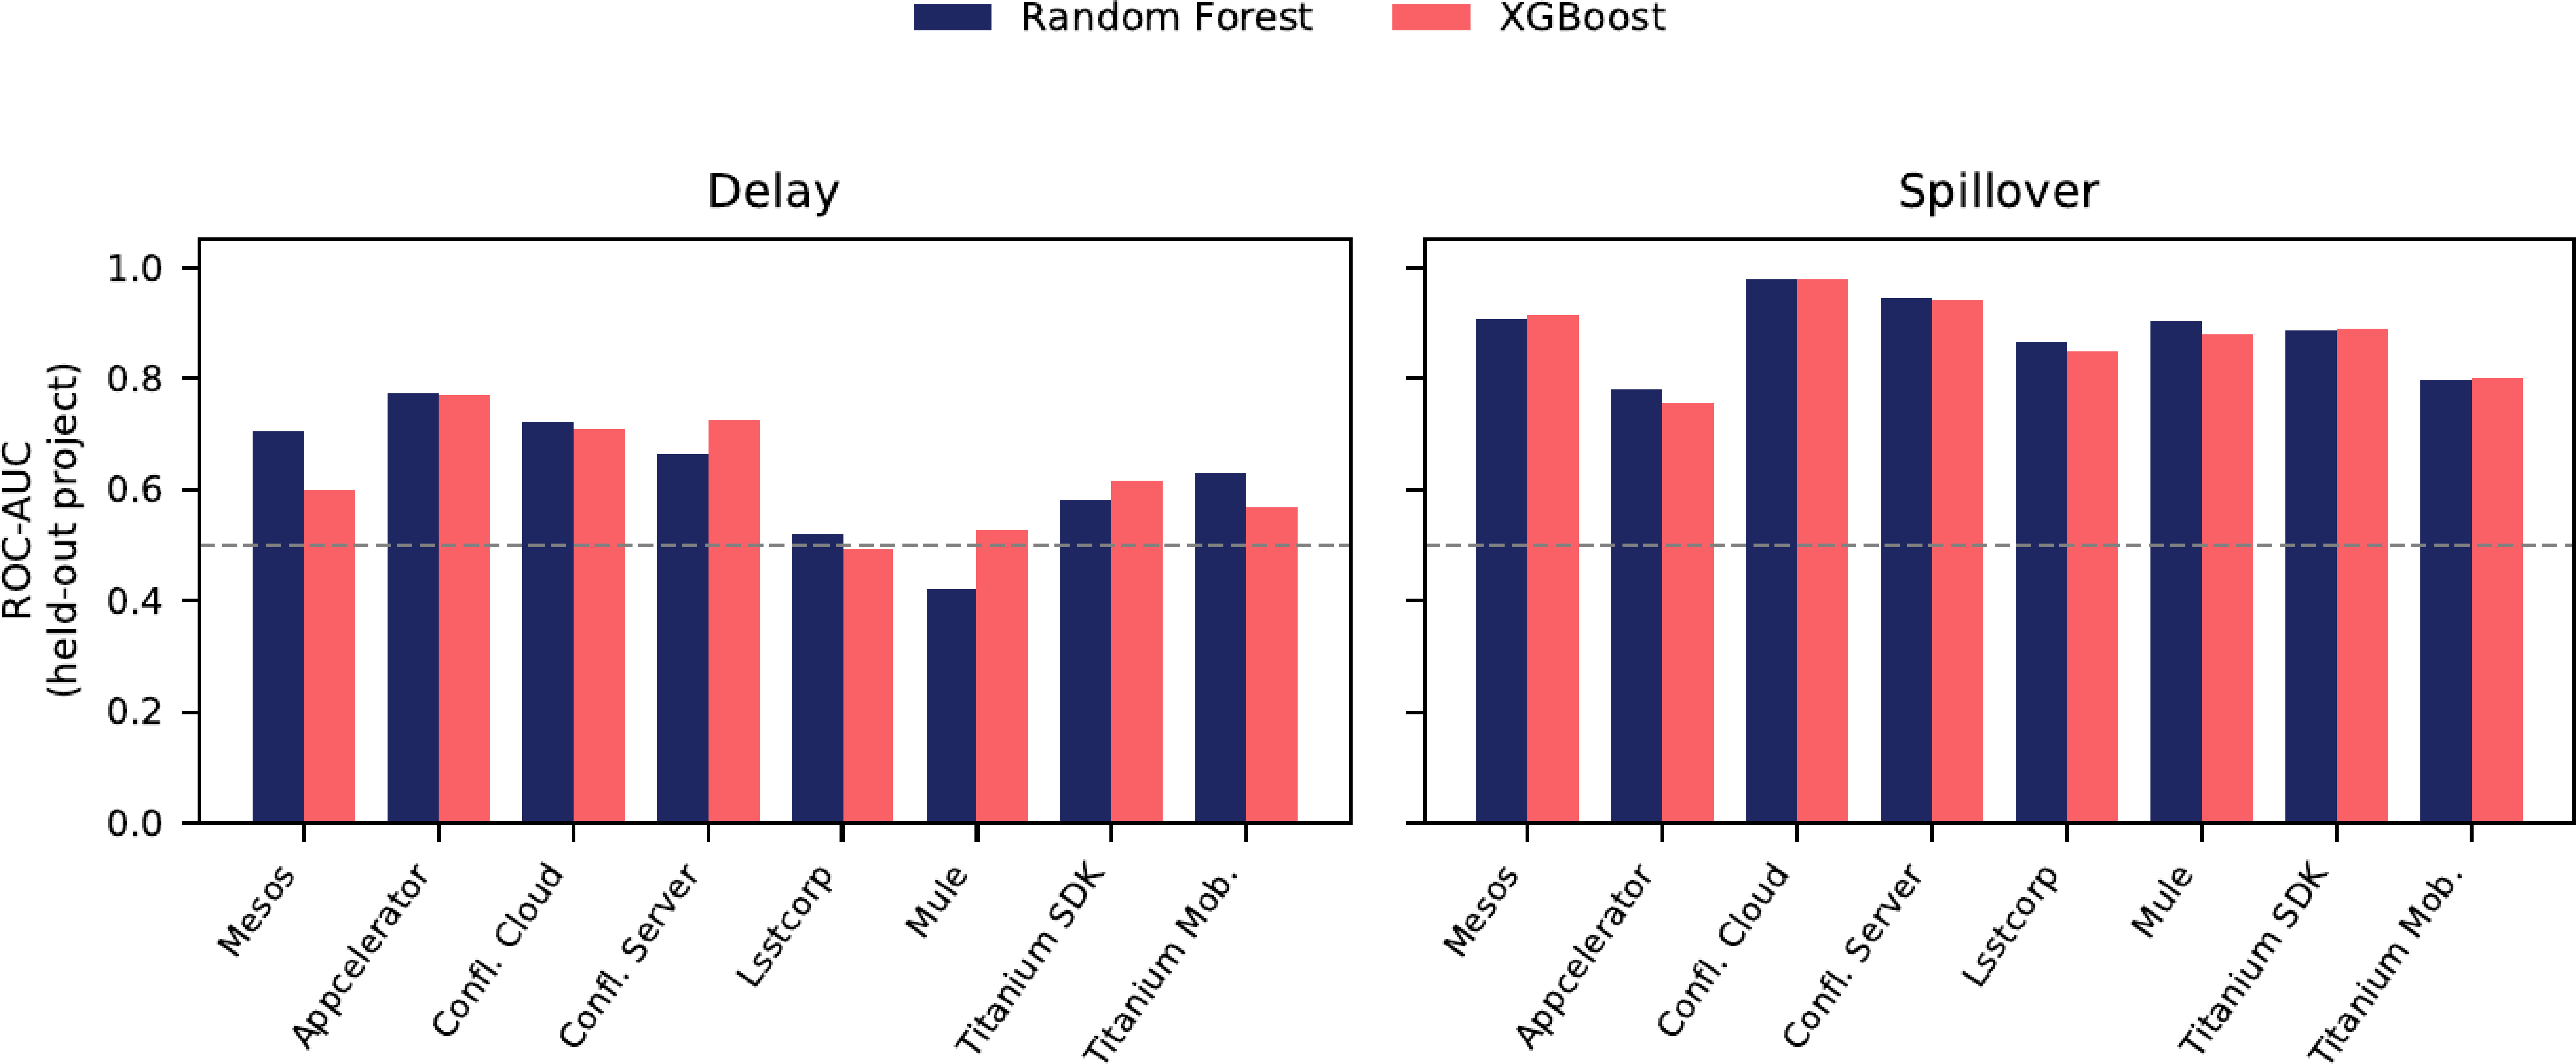
\includegraphics[width=0.93\columnwidth]{lopo_auc_by_project.png}
\caption{Held-out-project AUC by project.}
\label{fig:lopo}
\end{figure}

\subsection{Numeric outcomes}
\label{sec:numeric}

Table~\ref{tab:numeric} reports the numeric-outcome models under strict features.

\textbf{Issues completed} is the most predictable numeric outcome.
On the time split, the median-loss gradient booster achieves MAE 1.96 issues ($R^2 = 0.46$), compared with 2.10 for the scope-times-rate baseline ($R^2 = 0.42$).
The improvement is small: a bootstrap interval for the MAE difference is $[-0.31, +0.00]$, so the learned model does not significantly outperform the simple baseline on this split.
Across projects (LOPO), ridge regression reaches MAE 2.05 versus 2.14 for the baseline, and here the difference is marginally significant ($[-0.19, -0.00]$).
Scope is doing most of the work: multiplying committed issues by the team's historical completion rate is nearly as good as a learned model with all features.

\textbf{Carry share} is close to unpredictable.
All models have $R^2$ near zero.
The best learned model (median-loss gradient booster) reduces MAE from 0.232 (train median) to 0.201 on the time split and from 0.244 to 0.210 across projects.
Both reductions are significant by bootstrap (time split: $[-0.050, -0.012]$; LOPO: $[-0.059, -0.015]$), but the absolute improvement is small.
Knowing how much was committed and how the team has performed tells us little about what \emph{fraction} of the work will be left over.

\textbf{Days late} is heavy-tailed.
The median sprint closes 0.21 days late, the 90th percentile is 10 days, and the most extreme case is 2,603 days.
Models trained on squared error are worse than predicting the median: their MAE ranges from 3.7 to 4.1 versus 2.66 for the train median, because a few extreme sprints dominate the squared-error loss.
The median-loss gradient booster manages 2.48 on the time split (not significant versus the train median, $[-0.34, +0.03]$) and 3.13 across projects (significant versus 3.30, $[-0.30, -0.05]$).

\begin{table}[!htb]
\centering\scriptsize
\caption{Numeric outcomes (strict features), selected models}
\label{tab:numeric}
\setlength{\tabcolsep}{2.0pt}
\begin{tabular}{@{}llrrrr@{}}
\toprule
Task & Model & Protocol & n & MAE & $R^2$\\
\midrule
Issues done & Scope $\times$ rate & Time & 511 & 2.10 & .42\\
Issues done & GB median & Time & 511 & 1.96 & .46\\
Issues done & Scope $\times$ rate & LOPO & 1691 & 2.14 & .59\\
Issues done & Ridge & LOPO & 1691 & 2.05 & .67\\
\midrule
Carry share & Train median & Time & 511 & .232 & $-.02$\\
Carry share & GB median & Time & 511 & .201 & $-.11$\\
Carry share & Train median & LOPO & 1691 & .244 & $-.05$\\
Carry share & GB median & LOPO & 1691 & .210 & $-.05$\\
\midrule
Days late & Train median & Time & 786 & 2.66 & $-.12$\\
Days late & GB median & Time & 786 & 2.48 & $-.02$\\
Days late & Train median & LOPO & 2602 & 3.30 & $-.20$\\
Days late & GB median & LOPO & 2602 & 3.13 & $-.12$\\
\bottomrule
\end{tabular}
\end{table}

\subsection{Feature-group explanations}

Exact Shapley values decompose each model's test-set predictions into additive contributions from the seven feature groups.
Table~\ref{tab:shapley} reports each group's share of the total absolute attribution.

The results confirm and quantify the patterns visible in the classification comparison.
Late-closure predictions are driven by past lateness (38\%) and project identity (22\%), with scope contributing only 9\%.
The days-late prediction shows a similar pattern: project (26\%), past lateness (26\%), and sprint length (22\%) dominate.
In both cases, the model is learning team-specific timing habits, not reacting to how much work was committed.

For issues completed, scope accounts for 71\% of the attribution.
This is consistent with the near-parity between the scope-times-rate baseline and the learned model: a linear function of scope does most of the work.
Spillover shows a different composition: scope (41\%) and capacity (37\%) together account for 78\%, meaning that the model uses both how much was committed and how much the team typically finishes.

Carry share is the most distributed outcome: recent history (32\%), project (18\%), and capacity (12\%) lead, with no single group dominating.
This is consistent with its low predictability---no feature group provides a strong signal.

\begin{table}[!htb]
\centering\scriptsize
\caption{Shapley feature-group importance shares (\%)}
\label{tab:shapley}
\setlength{\tabcolsep}{2.0pt}
\begin{tabular}{@{}lrrrrr@{}}
\toprule
Group & Late cl. & Days late & Spill. & Iss.\ done & Carry\\
\midrule
Scope & 9 & 7 & 41 & 71 & 12\\
Sprint length & 13 & 22 & 2 & 3 & 9\\
Parallel & 2 & 2 & 1 & 2 & 10\\
Recent history & 4 & 12 & 12 & 12 & 32\\
Capacity & 12 & 5 & 37 & 6 & 12\\
Past lateness & 38 & 26 & 3 & 2 & 7\\
Project & 22 & 26 & 5 & 4 & 18\\
\bottomrule
\end{tabular}
\end{table}

\subsection{Sprint advisor evaluation}
\label{sec:advisor}

The advisor translates the fitted models into planning-time forecasts.
We evaluate two properties: interval coverage and the causal plausibility of what-if tables.

\textbf{Prediction intervals.}
The 80\% prediction intervals for issues completed cover 84\% of outcomes on the time split and 85\% across projects (LOPO), slightly above the nominal 80\%.
The intervals are about a third narrower than the scope-times-rate baseline (mean width 5.4 vs.\ 8.4 on the time split, and 6.6 vs.\ 9.5 across projects).
Coverage drops for sprints with 13 or more committed issues (70\% on the time split, 80\% across projects), reflecting the wider variance of larger sprints.

For days late, the 90th-percentile forecast is exceeded 10\% and 11\% of the time (time split and LOPO respectively), close to the nominal 10\%.

\textbf{Spillover probability} from the classification model has AUC 0.822 on the time split and 0.781 across projects.
The probability is well calibrated on the time split (top quartile: predicted 0.66, observed 0.66) but less so across projects (bottom quartile: predicted 0.16, observed 0.30), consistent with the LOPO variation in Section~\ref{sec:lopo}.

\textbf{What-if tables.}
The what-if table varies committed scope and reports expected outcomes.
However, these are observational associations, not causal effects.
The difference in carry share between the heaviest and lightest scope quartiles is 0.032, with a project-cluster 95\% bootstrap interval of $[-0.023, +0.084]$ that includes zero.
Late-closure probability differs by 0.056 between quartiles (interval $[-0.052, +0.164]$, also nonsignificant).
Within individual projects, the carry-share correlation with load is positive in only 2 of 8 projects, and late-closure correlation is positive in 5 of 8.
The table therefore describes what the fitted model expects, not what would happen if a team cut its scope.

\subsection{Provenance sensitivity}
\label{sec:provenance}

Table~\ref{tab:prov} restricts the conditional spillover analysis to subsets with observed change history.
Requiring observed Sprint history for every committed item cuts the sample to 1,174 sprints (356 test), where scope-only logistic regression holds at 0.875 AUC and random forest at 0.850.
Requiring both Sprint and Story Points history shrinks things to 358 sprints (110 test).
On this stricter subset, scope-only AUC drops to 0.772 and random forest to 0.652.
The smaller sample means less stable estimates, but the drop shows that provenance quality changes how hard the task looks---the static-fallback assumption is doing real work in the main analysis.

\begin{table}[!htb]
\centering\scriptsize
\caption{Conditional-spillover sensitivity to observed history}
\label{tab:prov}
\setlength{\tabcolsep}{2.4pt}
\begin{tabular}{@{}llrrrr@{}}
\toprule
Subset & Model & Test n & Pos. & F1 & AUC\\
\midrule
Observed Sprint & Scope LR & 356 & 335 & .719 & .875\\
Observed Sprint & RF & 356 & 335 & .875 & .850\\
Sprint + SP history & Scope LR & 110 & 94 & .652 & .772\\
Sprint + SP history & RF & 110 & 94 & .876 & .652\\
\bottomrule
\end{tabular}
\end{table}

\subsection{Leakage demonstrations}
\label{sec:leakage}

Table~\ref{tab:leak} shows how two common data-handling mistakes distort the results.
The mechanisms are:

\emph{Post-outcome feature leakage.}
We add the current sprint's own completion ratio (issues completed / committed) as a feature---a value available only after the sprint ends.
For spillover, this nearly-perfectly encodes the label: F1 jumps from 0.756 to 0.991.
For late closure, the effect is negligible (+0.010 F1), because completion ratio does not directly determine when the sprint was closed in Jira.
This asymmetry illustrates that leakage damage depends on the relationship between the leaked feature and the target, not just on the fact that future information was included.

\emph{Oversample-before-split leakage.}
We apply SMOTE to the full dataset before the train/test split rather than after, allowing synthetic copies of test-set sprints to enter training.
Late-closure F1 inflates from 0.457 to 0.646, a substantial artificial boost.
Spillover F1 barely changes (0.972 to 0.972), because the 94\% positive rate means SMOTE generates very few synthetic positives and the minority class is too small to produce visible duplicates in the test set.
Both mechanisms are easy to introduce accidentally; neither inflates results by a fixed amount.

\begin{table}[!htb]
\centering\scriptsize
\caption{Leakage demonstrations, F1 before and after the mistake}
\label{tab:leak}
\setlength{\tabcolsep}{2.6pt}
\begin{tabular}{@{}lllrr@{}}
\toprule
Outcome & Mechanism & Correct & Leaky & Change\\
\midrule
Late & Post-outcome feature & .463 & .473 & +.010\\
Late & Oversample before split & .457 & .646 & +.189\\
Spillover & Post-outcome feature & .756 & .991 & +.235\\
Spillover & Oversample before split & .972 & .972 & .000\\
\bottomrule
\end{tabular}
\end{table}

\subsection{Outcome-definition sensitivity}
The broad findings are not tied to one threshold.
For late closure, random-forest AUC is 0.696 with no grace day, 0.705 with the one-day definition, 0.685 with three days, and 0.626 with seven days.
In the full spillover population, requiring at least two or three unfinished issues produces AUCs of 0.984 and 0.980.
A story-point completion ratio below 0.8 gives 0.977 AUC.

%% ================================================================
\section{Discussion}

The five research questions receive different answers, which is the main point.

\textbf{RQ1 and RQ2: ranking signal and model complexity.}
Late closure carries moderate signal that depends on project context and team history (AUC 0.751 for gradient boosting, significant bootstrap interval above scope-only).
A scope-only model is essentially a coin flip for this outcome (AUC 0.530).
Spillover is easier to rank, but a three-variable scope model captures most of the signal (AUC 0.885), and richer models do not improve.
The practical implication is that for spillover, all a prediction system needs to know is how many issues and story points were committed and how long the sprint is.

\textbf{RQ3: strict history features.}
Accounting for parallel-sprint timing improves late-closure prediction---most notably in LOPO, where logistic regression jumps from 0.542 to 0.629.
The improvement is smaller on the time split (+0.025 for gradient boosting) but consistent across models.
Spillover is unaffected because scope, which is identical in both feature sets, dominates that outcome.
This validates the concern that naive ``prior sprint'' features can leak information from unfinished concurrent sprints.

\textbf{RQ4: explanations.}
Shapley values make the story quantitative.
Late closure is a team-habits outcome: past lateness (38\%) and project (22\%) together account for 60\% of the attribution, while scope accounts for 9\%.
Issues completed is a scope-arithmetic outcome: 71\% of the attribution comes from committed scope.
Carry share is the most distributed and least predictable outcome.
These explanations are consistent with the classification and regression results, which makes both the models and the explanations easier to trust.

\textbf{RQ5: planning-time forecasts.}
The advisor's 80\% intervals for issues completed are calibrated (84--85\% coverage) and a third narrower than a simple baseline.
The days-late 90th-percentile forecasts are well calibrated (10--11\% exceedance).
However, the what-if tables are not causal: heavier scope does not significantly predict higher carryover or late closure across projects.
This means the advisor is useful for setting expectations (``if you commit 15 issues, expect to finish 10--12'') but not for prescribing scope changes (``cut to 10 issues and you'll close on time'').

\textbf{LOPO variation.}
LOPO results vary from 0.531 to 0.780 for late closure and 0.706 to 0.950 for spillover.
This variation is not noise---it reflects genuine differences in project practices, team size, and how consistently teams use sprint closure in Jira.
Projects with extreme or very uniform outcome rates (Mule at 19.2\% late, Lsstcorp at 98.4\% spillover) are harder to rank because there is less variation to discriminate.
Any deployment would need project-local calibration.

\textbf{What this does not show.}
The analysis ranks historical sprints under stated assumptions---it does not demonstrate that acting on scores would improve delivery, that the models would calibrate in enterprise settings, or that cutting scope reduces risk.
A sensible next step would be a silent prospective deployment: generate scores without letting them influence team behavior, calibrate locally, and only then consider intervention.

%% ================================================================
\section{Threats to Validity}

\textit{Construct validity.}
Jira's completion timestamp marks when the sprint was closed, not necessarily when the work finished.
Late closure is therefore an administrative outcome.
The spillover label captures only whether at least one item was unresolved by the planned end---not the severity or importance of the remaining work.
Neither label should be treated as a measure of team performance.

\textit{Reconstruction validity.}
Missing Sprint or Story Points history is handled with a static fallback.
The provenance tables and sensitivity analyses show how much the results depend on that choice, but cannot recover events that were never recorded.
Strict history features reduce one form of temporal contamination (parallel-sprint timing) but cannot guarantee that the reconstructed state matches the team's actual planning-time knowledge.

\textit{Evaluation validity.}
Eight projects produce wide project-level uncertainty.
LOPO retains local history from the held-out project and should be interpreted as transfer of the learned rule rather than a true cold start.
Thresholded metrics are affected by prevalence, especially for spillover.
Shapley values describe the fitted models' behavior, not causal mechanisms.

\textit{External validity.}
The projects are open-source Jira projects with public issue trackers.
Enterprise teams may differ in staffing, backlog practice, administrative sprint closure, and estimation culture.
Absolute performance numbers should not be transported without local validation.

\balance
%% ================================================================
\section{Reproducibility}

The full pipeline---data preparation, modeling, explanations, and advisor---is available at \url{https://github.com/hani-ziad/AddAI_MaryamHani_Assign1}.
Three CSV exports (Sprint, Issue, and Change\_Log) feed the reconstruction.
Phase~1 results are regenerated by \texttt{scripts.run\_baseline}, \texttt{scripts.run\_assignment\_comparison}, and \texttt{scripts.run\_validation\_sensitivity\_analyses}.
Phase~2 results are regenerated by \texttt{experiments.run\_all}.
Automated tests cover labels, cold starts, planning snapshots, feature construction, Shapley axioms, and leakage cases.
The seed is fixed at 42 throughout; results are deterministic within ordinary numerical tolerance.
The recorded environment was Python~3.13.5, NumPy~2.3.5, pandas~2.2.3, and scikit-learn~1.8.0.

%% ================================================================
\section{Conclusion}

Reconstructed Jira history contains measurable signal for sprint-start outcomes, but the signal is narrower and more outcome-specific than a generic ``sprint risk'' claim.
Late closure is moderately discriminable (AUC 0.751 with gradient boosting and strict features) and depends on team habits---past lateness and project identity account for 60\% of the Shapley attribution, while scope contributes 9\%.
Spillover is easier to rank (scope-only AUC 0.885) but harder to act on: the near-ceiling prevalence (94\%) means that committing any scope almost guarantees unfinished work, and observational evidence does not support reducing scope as a remedy.
Strict history features that respect parallel-sprint timing improve late-closure prediction, particularly across projects (LOPO logistic regression: 0.542 to 0.629), and the sprint advisor's prediction intervals are calibrated and narrower than simple baselines.
Numeric outcomes confirm the scope-arithmetic nature of issues completed ($R^2 = 0.46$, with scope accounting for 71\% of the explanation) and the near-unpredictability of carry share ($R^2 \approx 0$).
The practical value of these models remains a question for prospective validation with real teams, project-local calibration, and careful separation of observational ranking from causal advice.

%% ================================================================
\begin{thebibliography}{12}
\bibitem{tawosi2022} V. Tawosi, A. Al-Subaihin, R. Moussa, and F. Sarro, ``A versatile dataset of agile open source software projects,'' in \emph{Proc. 19th Int. Conf. Mining Software Repositories}, 2022, pp. 707--711.

\bibitem{tawosi2023} V. Tawosi, A. Al-Subaihin, and F. Sarro, ``Agile effort estimation: Have we solved the problem yet? Insights from a replication study,'' \emph{IEEE Trans. Softw. Eng.}, vol. 49, no. 6, pp. 3418--3439, 2023.

\bibitem{choetkiertikul2019} M. Choetkiertikul, H. K. Dam, T. Tran, T. T. M. Pham, A. Ghose, and T. Menzies, ``A deep learning model for estimating story points,'' \emph{IEEE Trans. Softw. Eng.}, vol. 45, no. 7, pp. 637--656, 2019.

\bibitem{shankar2026} S. P. Shankar, S. S. Chaudhari, V. Mishra, and T. Stephan, ``Intelligent techniques for predictive analytics in Agile software development,'' \emph{Scientific Reports}, vol. 16, 2026.

\bibitem{perezcastillo2024} Y. J. P\'{e}rez Castillo, S. D. Orantes Jim\'{e}nez, and P. O. Letelier Torres, ``Sprint management in Agile approach: Progress and velocity evaluation applying machine learning,'' \emph{Information}, vol. 15, no. 11, 2024.

\bibitem{obike2025} P. G. Obike, V. E. Ekong, and O. U. Obot, ``A novel scoring-based Agile sprint deliverability prediction and prioritization using machine learning,'' \emph{Int. J. Comput. Appl.}, vol. 187, no. 49, 2025.

\bibitem{almalki2025} S. S. Almalki, ``AI-driven decision support systems in Agile software project management,'' \emph{Systems}, vol. 13, no. 3, 2025.

\bibitem{lundberg2017} S. M. Lundberg and S.-I. Lee, ``A unified approach to interpreting model predictions,'' in \emph{Advances in Neural Information Processing Systems}, vol. 30, 2017.

\bibitem{molnar2022} C. Molnar, \emph{Interpretable Machine Learning: A Guide for Making Black Box Models Explainable}, 2nd ed., 2022. [Online]. Available: \url{https://christophm.github.io/interpretable-ml-book/}

\bibitem{xgboost2016} T. Chen and C. Guestrin, ``XGBoost: A scalable tree boosting system,'' in \emph{Proc. ACM SIGKDD}, 2016, pp. 785--794.

\bibitem{rf2001} L. Breiman, ``Random forests,'' \emph{Mach. Learn.}, vol. 45, no. 1, pp. 5--32, 2001.

\bibitem{sklearn2011} F. Pedregosa et al., ``Scikit-learn: Machine learning in Python,'' \emph{J. Mach. Learn. Res.}, vol. 12, pp. 2825--2830, 2011.
\end{thebibliography}
\end{document}
